\hypertarget{planetoideditor}{\section{Planetoid-Editor}}

\begin{figure}[H]
	\centering
	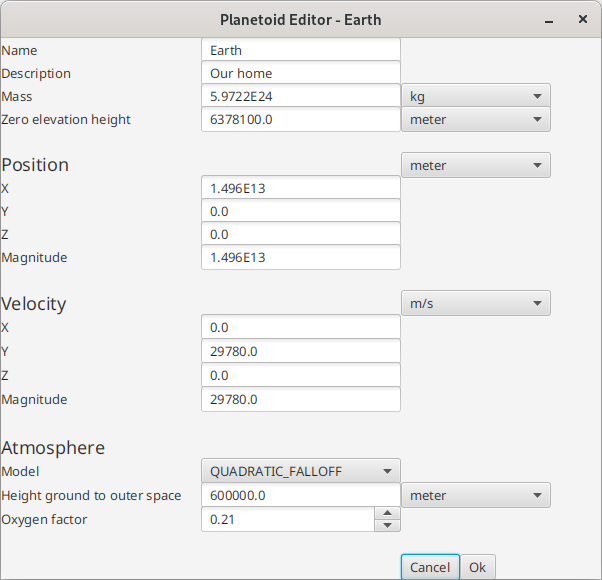
\includegraphics[width=12cm]{res/planetoideditor.png}
	\caption{GUI Planetoid-Editor mit Annotation. Planetoid Erde geöffnet.}
\end{figure}

\begin{enumerate}[noitemsep]
	\item Planetoidname
	\item Kurzbeschreibung
	\item Masse mit Grössenumrechnung
	\item Nullpunkthöhe mit Grössenumrechnung
	\item Positionsdaten
	\item Geschwindigkeitsdaten
	\item Atmosphärenmodel
	\item Atmosphärenhöhe bis Vakuum mit Grössenumrechnung
	\item Sauerstoffanteilsfaktor
	\item Cancel: Bearbeitung ohne Speicherung abbrechen
	\item Ok: Speichern und schliessen
\end{enumerate}

\subsection{Grundlagen}
Der Planetoid-Editor erlaubt das editieren der Simulationswerte eines Planetoiden. Position und Geschwindigkeit können direkt in den jeweiligen Vektordimensionen (X, Y, Z) gepflegt und bei Bedarf mit dem Längen-Feld (Magnitude) skaliert werden. Für übersichtlichere Darstellung können die Zahlenwerte dynamisch mit dem danebenstehenden Grössenumrechnungs-Dropdown umgewandelt werden. Eingaben werden beim Speichern überprüft. Im Fehlerfall wird die Speicherung verhindert und mit dem Feldverweis and den Benutzer gemeldet.

\subsection{Editieren eines Vektors}


\subsection{Speichern des Planetoiden}
Klicken sie auf Ok.
Ist eine Eingabe fehlerhaft so erscheint eine Fehlermeldung mit der Feldbezeichnung und Fehlerbeschreibung.

\begin{figure}[H]
	\centering
	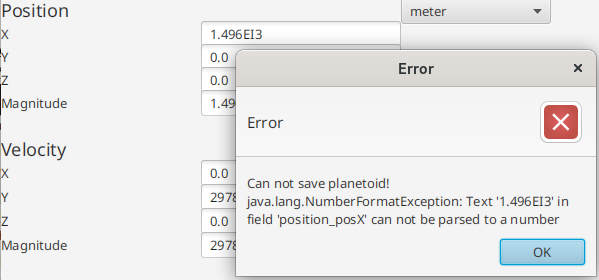
\includegraphics[width=12cm]{res/planetoidsaveerror.png}
	\caption[Planetoid-Editor Fehlermeldungsbeispiel]{Planetoid-Editor Fehlermeldung: Buchstabe 'I' im Zahlenfeld}
\end{figure}

Können alle Eingaben verarbeitet werden, wird der Planetoid gespeichert und der Planetoid-Editor wird geschlossen.